\chapter{Remarks on the Data}
\label{ch:data}

In this Chapter several properties of the data at hand will be explored.

%\section{Data Transformations}

Due to specific interests on the particular contents of tables, no exact replica of each table is to be found in the output database.
Instead, every table is processed before being sent to its destination, in order to compose the output database to be most useful to the marketing team, whilst considering storage efficiency.
In particular, three classes of tables will be introduced, depending on the nature of the transformation carried out: plain, time-traveled, and aggregated.

Plain tables are the simplest to discuss since they can be defined as a projection over a subset $S$ of the source table's columns; formally, for some plain table $\omega$:
$$
\dest{\omega} := \pi_{S} \big( \source{\omega} \big) \; .
$$

Aggregated and time-traveled tables instead require a more detailed discussion, thus let us introduce them here and discuss them in detail in \S \ref{sec:aggregations} and Chapter \ref{ch:timetravel} respectively.
As the name suggests, aggregated tables are defined as an aggregation of data contained in the source table.
Time-traveled tables are a peculiar representation of their respective source table: they not only retain a current view of the source table, but also store all changes that have occurred to it.


\section{Aggregated Tables}
\label{sec:aggregations}

In this Section, the four aggregated tables that are considered in this CDC system will be presented and the destination tables will be defined in terms of Relational Algebra queries performed on the source tables.
Extensive use of the grouping extension to Relational Algebra introduced in \S \ref{sec:notation-aggregation} will be made.
In addition, several references to code implementing the following aggregations, can be found in this Section.

\begin{align}\label{agg:eta}
	&\dest{\eta} := \gamma_{\text{user, day, class, count(*)} \rightarrow n \text{,} \sum (\text{cost}) \rightarrow C} \bigl( \\
	&\ind \sigma_{\isfinal{*}}\bigl( \source{\eta} \bigr) \nonumber\\
	&\bigr) \nonumber
\end{align}

\begin{align}\label{agg:theta}
	&\dest{\theta} := \gamma_{\text{user, day, count} (*) \rightarrow n} \bigl( \\
	&\ind \sigma_{\isfinal{*}}\bigl( \source{\theta} \bigr) \nonumber \\
	&\bigr) \nonumber
\end{align}

Let us begin with two very similar aggregations.
For these tables, we are aggregating operations count and cost based on the user who performed them, the day, and the class of operation, with the latter only being relevant for $\eta$.

For these aggregations, let us introduce a new function used to filter out data change events emitted from non-finalized rows: the function $\isfinal{*}$ yields truth if the evaluated row will not undergo changes anymore, and it is thus finalized.
This aspect is important because if non finalized rows were considered, they would be counted more than once towards the aggregation.
For instance, say that some row goes from state A to B: two data change events would be emitted and $n$ would be increased by 2, which is not the intended behavior.
In Listings \ref{src:eu.spaziodati.metrics/streams/etaStream.scala}, line 22, and \ref{src:eu.spaziodati.metrics/streams/thetaStream.scala}, line 23, you can see this function implemented: rows that are not in a \emph{done} or \emph{error} state are not finalized, thus they are filtered out.

In Figure \ref{fig:aggregation-processing} a visualization of Query (\ref{agg:eta})'s aggregation processing is presented in terms of Kafka Streams APIs used.
In Kafka's terminology, the content of this Figure is the stream's \emph{topology}; in fact, the data for producing Figure \ref{fig:aggregation-processing} was obtained making again use of its APIs.\footnote{%
	See \cite[Topology\#describe]{kafka-javadocs}: 	\url{https://kafka.apache.org/27/javadoc/org/apache/kafka/streams/Topology.html\#describe--}\lastvisited
}
Very similar results were obtained for all other aggregations in this Section.

Comparison of said Figure with code in Listing \ref{src:eu.spaziodati.metrics/streams/etaStream.scala} yields a direct relationship between methods used and the topology description.
In fact they are lines 10 -- 63 that generate the above topology.
Let us make a detailed comparison only for table $\eta$: other tables perform very similar operations.

Consider line 12: the \texttt{filter} method is the first filter step in the topology, which implements $\sigma_{\isfinal{*}}$, along with other required technical checks that we may leave out of the discussion.

Going further, on line 24 the \texttt{map} method is reflected as the next step after \texttt{filter} also on Figure \ref{fig:aggregation-processing}, again this is used for primarily technical reasons.

Then, the \texttt{groupBy} method on line 29, which acts in a similar fashion as SQL's \texttt{GROUP BY} clause, is expanded into three steps which eventually output into a new repartitioning topic that Kafka Streams creates on its own.
It is used to allow a new keying of the stream, i.e. the source's primary-key is exchanged for the grouping keys.\footnote{%
	A computation similar to Definitions (\ref{def:G}), and (\ref{def:G-keys}).
}

Next, the \texttt{aggregate} method, on line 40, acts similarly to operator $\sigma^*$\footnote{%
	See Definition (\ref{def:sigma*}).
} and actually carries out the computation of counting records and summing the cost.

On line 57, the following method \texttt{toStream} may seem strange, given that we have since been operating on a stream.
Its necessity comes from the fact that Kafka when performing the repartitioning caused by \texttt{groupBy}, represents the new data as a table, in order to efficiently carry out the upcoming computations, making again use of the duality between streams and tables.
At this point, there is no longer the need to do so, hence the method call.

Finally on lines 58 -- 61, \texttt{mapValues} renders the data in a manner that the Kafka Connect Sink developed can understand and use to transfer data to the output database, and the \texttt{to} method indicates which topic to output the computed records to.

In summary, we have shown how Query (\ref{agg:eta}) is transformed into code for Kafka Streams.

\begin{figure}
	\centering
	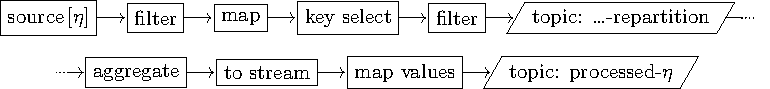
\includegraphics[width=\linewidth]{figures/data/aggregation-processing}
	\caption{Processing of aggregation Query (\ref{agg:eta}) in terms of Kafka Streams APIs used.}
	\label{fig:aggregation-processing}
\end{figure}

\begin{align}\label{agg:kappa}
	&\dest{\kappa} := \gamma_{\text{user, day, class, subclass,} \sum(\text{cost}) \rightarrow C} \bigl( \\
	&\ind \sigma_{\text{class} = \texttt{'c'}}\bigl( \source{\kappa} \bigr) \nonumber \\
	&\bigr) \nonumber
\end{align}

One peculiar aspect of the $\dest{\kappa}$ table is the presence of a \emph{class} attribute, which appears in Query (\ref{agg:kappa}).
From the query itself one can rightly argue that since only rows with \emph{class} $= \texttt{'c'}$ are kept, the attribute should be discarded altogether: since it's always the same value, it bears no meaningful data.
The rationale for keeping the \emph{class} attribute in the output database was that possible future interventions on the system, guided by a change of interest from the marketing team, would require said attribute.
Thus, it was decided to have it in the destination table to facilitate possible future works.

\begin{align}\label{agg:lambda}
	&\dest{\lambda} := \pi_{\dest{\alpha}.\text{id} \text{, day, class, } n} \bigl(\\
	&\ind \dest{\alpha} \bowtie \gamma_{\text{email, day, class, count} (*) \rightarrow n} \bigl( \nonumber\\
	&\ind\ind \source{\lambda} \nonumber\\
	&\bigr)\bigr) \nonumber
\end{align}

The $\lambda$ table arguably bears the most interesting aggregation query.
Not only source data is aggregated, but it is also enriched after aggregation: see join operation in second line of Query (\ref{agg:lambda}).

The motive for this operation lies in the fact that $\source{\lambda}$, for historical reasons, holds the user's email instead of its identifier.
In order to have more coherence in the output database, it was decided that in the processing of this table, the email would be converted into an identifier.
This is reasonable because a single email is ever only associated with one user.

From the query, $\dest{\alpha}$ is used to perform the join operation.
This is formally incorrect: as one might expect, if a user is registered and the associated data change has not been processed by the CDC system before a record from $\source{\lambda}$ is processed, then the join operation would fail.

While this is true, one should consider that it is very unrealistic.
In fact, because of Atoka's application logic, there is a sensible temporal distance between the registration of a user and the first time a record can be emitted from $\source{\lambda}$ pertaining that user.
In addition, performing the join query on the source database, which would yield a formally correct operation, would impact the data source's performance, which is undesirable.
Therefore, on the grounds of common sense, it was decided to use the more efficient option.


\section{On Constraints}

Enforcing constraints on data is meant to provide consistency to a database.
That is, by restricting the set of possible values down to a more sensible subset, the data contained in the database can make more sense.
For instance, we may not allow to have users under legal age to be represented in a database, thus we would reduce an \emph{age} attribute from the set of integers down to the set of integers greater than or equal to 18.

With regards to relational databases the constraints generally considered are the following:

\begin{enumerate}
	\item uniqueness (including primary-key),
	\item conditional (including non-null), and
	\item referential integrity (foreign-key).
\end{enumerate}

Let us discuss how these constraints are carried from the data source over to the output database, which is a property we are interested in.
To do so formally, let the following be assumed:

\begin{axiom}\label{axiom:source-consistency}
	$\source{*}$ is consistent.\footnote{%
		Meaning: every constraint which has been set at schema definition, holds.
		The source database's consistency should be assumed because a database replication can only be as consistent as the original database, i.e. there is no sensible mechanism to reach data consistency, starting from inconsistent data.
		Additionally, such is safe to assume, since the database constraints are checked at the source by the PostgreSQL server.
	}
\end{axiom}

Considering Assumption (\ref{axiom:source-consistency}), let us examine the three constraint classes enumerated above.
With regards to the first two, the fact that they are carried over to the output database really is a corollary to Assumption (1).
Consider some table $\omega$: if the constraint holds for $\source{\omega}$ and the data contained in records streamed is received unmodified,\footnote{%
	This is true for every table that doesn't undergo any processing in the stream, therefore it is not true for aggregated tables.
	Nonetheless, given the above definition queries, we can state that there is no modification of values, thus the following reasoning holds for aggregated tables as well.
	This is also true for time-traveled tables.
} then for each unique value in some attribute of $\source{\omega}$ there is a unique value in $\dest{\omega}$.
Similarly, for each condition on any value in some attribute of $\source{\omega}$, that condition holds for any respective value in $\dest{\omega}$.

With regards to the referential integrity (or foreign-key) constraint, the fact that it holds in the output database is no corollary to Assumption (1).
Considering also the amount of foreign-key relations between the tables we are interested in, depicted in Figure \ref{fig:fk-relations}, let us have a lengthier discussion.

\begin{figure}
	\centering
	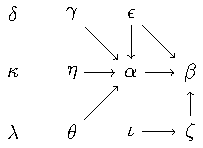
\includegraphics[width=0.3\linewidth]{figures/data/fk-relations}
	\caption{Foreign Key Relational Dependencies.}
	\label{fig:fk-relations}
\end{figure}


\subsection{On Foreign Key Constraints}
\label{sec:foreign-key}

One particular aspect on the processing of streams is that they are processed in parallel.
That is, records pertaining to one table are processed in succession,\footnote{%
	In particular, they have to: one of the core principles expressed in \S \ref{sec:tables-streams} is that data change events emitted from one table are processed sequentially, otherwise their application to the destination table is not guaranteed to be consistent with the source.
} but records pertaining to different tables are processed independently of each other, possibly at the same time.

The problem, depicted in Figure \ref{fig:fk-stream}, which arises with foreign-keys is that, given the parallelism of streams processing, a record may fail to be processed on the grounds that a referenced value has not been processed yet, thus resulting in an error raised by the output database.
Therefore, we want records that have this particular requirement to be processed after those records that are required for the destination database's consistency.

Formally, let us denote with $r(f^*)$ a record that contains a reference to some attribute $f$ which is part of another relation, and let $s(f)$ be the record containing the value in attribute $f$ that is referenced in $r$.
A processing failure on $r$, that is due to a foreign-key constraint, means that the database system is refusing to process $r$ on grounds that the referenced value $f^*$ is not to be found in the relation containing attribute $f$.

\begin{proposition}\label{prop:fk}
	Let $r(f^*)$ be a record containing a foreign-key constraint on $f$.
	Let $r$ fail to be processed due to the constraint on $f$.
	Then
	\begin{enumerate}
		\item $s(f)$ is an existing record containing the value referenced in $r(f^*)$; and
		\item $s(f)$ is in the unprocessed part of the stream.
	\end{enumerate}
\end{proposition}
\begin{proof}
	(1) Let $\source{\omega}$ be the relation which emitted record $r$ and $\source{\psi}$ the table referenced in $\source{\omega}$ that contains attribute $f$.
	For a record to be emitted from a table, there has to be a data change contained in a committed transaction that has taken place in the data source.
	A transaction can only be committed if every functional dependency within it is satisfied.
	Thus, the transaction that caused the emission of $r$, must have had the functional dependency on $f$ satisfied.
	
	It follows that $\source{\psi}$ contains the value referenced in $r(f^*)$, otherwise $\source{*}$ would not be consistent.\footnote{Cf. Assumption (\ref{axiom:source-consistency}).}
	Thus, there must be a data change event that contains the value referenced in $r$, in other words, $\exists s(f)$ record emitted from $\source{\psi}$ that satisfies reference $f^*$.
	
	(2) Since $r(f^*)$ is failing to be processed due to the foreign-key constraint, $s(f)$ cannot be in the portion of stream that has already been processed, else there would be no failure.
\end{proof}

\begin{figure}
	\centering
	\begin{tabular}{p{0.45\textwidth} p{0.45\textwidth}}
		\vspace{0pt} 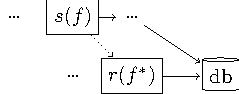
\includegraphics[width=0.4\textwidth]{figures/data/fk-stream} &
		\vspace{0pt} 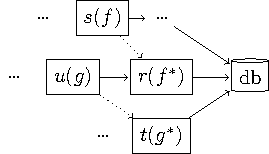
\includegraphics[width=0.44\textwidth]{figures/data/fk-stream-recurrence} \\
		(a) & (b)
	\end{tabular}
	\caption{(a) Depiction of the foreign-key problem. (b) The same problem recurred.}
	\label{fig:fk-stream}
\end{figure}

Proposition (\ref{prop:fk}) tells us that a solution can be found, since the record required does exist and is in fact in one of the streams.

Logically, the solution to this problem is to be found in topological sorting algorithms,\footnote{%
	See for reference \cite[\S 9.5.8]{montry}.
} since the various records that present this issue would yield a dependency graph when combined.
In practical terms, since data change events related to each individual table are streamed in parallel, one solution to this problem could be to have the problematic streams hold processing until the referenced records are processed, assuming that progress on every other stream is never halted.
Though, this causes a notable degradation of the CDC system's performance.

After careful consideration, it was decided to relax the requirement of having foreign key constraints on the destination database, for the sake of performance.
The output database would therefore not guarantee consistency (only in so far as foreign-keys are concerned), instead it would guarantee an \emph{eventual} consistency.
That is, assuming progress of every stream, given Proposition (\ref{prop:fk}), the output database would become consistent once all records are processed.
%Introduction of further records would then reiterate the questioning of consistency which will eventually be restored again.
